\clearpage
\subsection{MSVC: x86 + \olly}
\index{\olly}

\RU{Тут даже проще}\EN{Things are even simpler here}:

\begin{figure}[H]
\centering
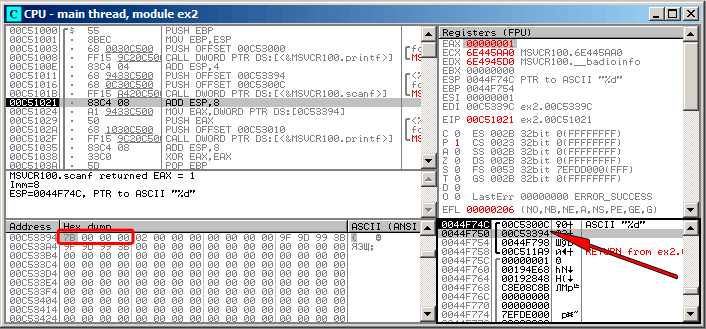
\includegraphics[scale=\FigScale]{patterns/04_scanf/2_global/ex2_olly_1.png}
\caption{\olly: \RU{после исполнения \scanf}\EN{after \scanf execution}}
\label{fig:scanf_ex2_olly_1}
\end{figure}

\RU{Переменная хранится в сегменте данных.}
\EN{The variable is located in the data segment.}
\RU{Кстати, после исполнения инструкции \PUSH (заталкивающей адрес $x$) адрес появится в стеке, 
и на этом элементе можно нажать правой кнопкой, выбрать ``Follow in dump''.}
\EN{After the \PUSH instruction (pushing the address of $x$) gets executed, 
the address appears in the stack window. Right-click on that row and select ``Follow in dump''.}
\RU{И в окне памяти слева появится эта переменная.}
\EN{The variable will appear in the memory window on the left.}

\RU{После того как в консоли введем 123, здесь появится}\EN{After we have entered 123 in the console,} 
\TT{0x7B}\EN{ appears in the memory window (see the highlighted screenshot regions)}.

\RU{Почему самый первый байт это}\EN{But why is the first byte} \TT{7B}?
\RU{По логике вещей, здесь должно было бы быть}\EN{Thinking logically,} \TT{00 00 00 7B}\EN{ should be
there}.
\RU{Это называется}\EN{The cause for this is referred as } \gls{endianness}, \RU{и в x86 принят формат}\EN{and x86 uses }\IT{little-endian}.
\RU{Это означает что в начале записывается самый младший байт, а заканчивается самым старшим байтом}
\EN{This implies that the lowest byte is written first, and the highest written last}.
\RU{Больше об этом}\EN{Read more about it at}: \myref{sec:endianness}.

\RU{Позже, из этого места в памяти, 32-битное значение загружается в \EAX и передается в}
\EN{Back to the example, the 32-bit value is loaded from this memory address into \EAX and passed to} \printf.

\RU{Адрес переменной $x$ в памяти}\EN{The memory address of $x$ is} \TT{0x00C53394}.

\clearpage
\RU{В \olly{} мы можем посмотреть карту памяти процесса (Alt-M) и увидим, что этот адрес
внутри PE-сегмента \TT{.data} нашей программы}
\EN{In \olly we can review the process memory map (Alt-M)
and we can see that this address is inside the \TT{.data} PE-segment of our program}:

\begin{figure}[H]
\centering
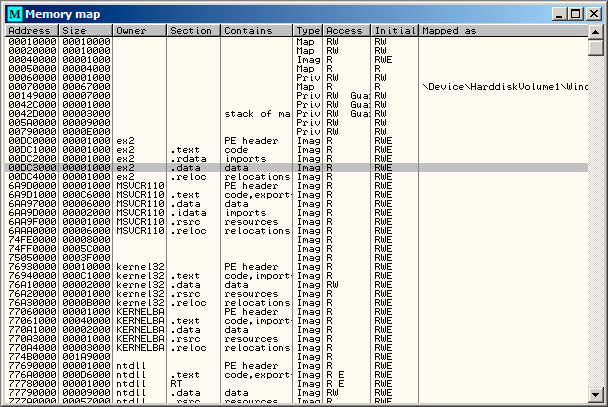
\includegraphics[scale=\FigScale]{patterns/04_scanf/2_global/ex2_olly_2.png}
\caption{\olly: \RU{карта памяти процесса}\EN{process memory map}}
\label{fig:scanf_ex2_olly_2}
\end{figure}
